\section{Case Study: ThingSat}
\label{sec:case-study}

\subsection{Overview}
% \paragraph*{Mission Goal:} in-orbit observation of glaciers in Europe and in Polynesia.
% \paragraph*{Approach}: rent "rack" space as payload on a CubeSat (SatRevolution).

The Thingsat project~\cite{git:thingsat-repo} aims to benchmark the LoRa links in the context of
space-ground communication for several frequency bands and demonstrate the
effectiveness of that technology inside a LEO (Low Earth Orbit) cubesat. 

Thus we designed a space electronic board with two LoRa transceivers and a patch
antenna operating in 868MHz and 2.4GHz. This payload is hosted in a shared 3U
CubeSat - \href{https://space.skyrocket.de/doc_sdat/stork-1.htm}{STORK-1} from
the polish start-up \href{https://www.satrevolution.com/}{SatRevolution}. The
cubesat was launched on January 13th, 2022 on a near-polar orbit at an
altitude of 525 km (See
\href{https://www.n2yo.com/database/?q=STORK-1\#results}{Two-Line Elements}).

This project can be adapted to a wide range of use cases, for players as varied
as Earth science researchers (e.g. Ocean levels, melting of glaciers, pirate
fishing...) and companies with widely dispersed objects (e.g. The monitoring of
tank ships). 

\begin{figure}[t]
    \centering
    \includegraphics[width=0.5\textwidth]{Figures/thingsat-dtn.png}
    \caption{ThingSat in-orbit communication patterns.}
    \label{fig:thingsat-comm}
\end{figure}

To able to test several use-cases illustrated in figure \ref{fig:thingsat-comm},
the Thingsat payload may act in turns as either i) a Sat-IoT end-device (ED)
that will send Lora frames to terrestrial LoRaWAN gateways or Thingsat ground
stations (GS) or ii) an in-orbit LoRa sniffer or iii) a store-carry-and-forward
LoRa gateway.

The first and second scenarios allows to benchmark ground-space LoRa links by
making statistics over multiple sent/received frames. In the third and more
complex scenario, the satellite stores packets received from GS/ED and deliver
them once GS/ED destinations are inside the footprint of the satellite.

% \paragraph*{High-level overview of Segments}

\subsection{Distributed System Architecture}

The figure \ref{fig:archi} generalizes the Thingsat context by giving an
overview of a cubesat ecosystem where the interaction with a hosted payload go
through an unstrusted part.

\begin{figure}[ht]
    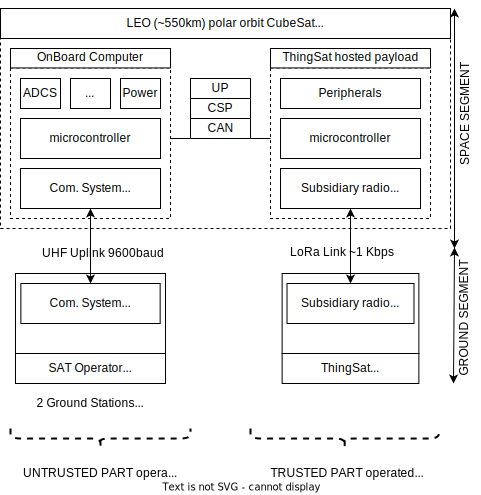
\includegraphics[width=0.5\textwidth]{Figures/globecom-thingsat.jpg}
    \caption{The cubesat ecosystem}
    \label{fig:archi}
\end{figure}

% \paragraph*{Space Segment Description}
The \textit{Space Segment}  comprises especially the OBC and payloads. The OBC
consists of a microcontroller with all its subsystems to operate the cubesat :
the Attitude Determination and Control System, the communication subsystems
(UHF/VHF/S-band for uplink/downlink + antennas), the power subsystem (Battery
Management, Energy Harvesting with Solar Panels, Auxiliary Power Supply). The
payload designed for the Thingsat project embeds one
\href{https://www.semtech.com/products/wireless-rf/lora-gateways/sx1302}{Semtech
SX1302 concentrator} for communications on the 863-870 MHz band and one
\href{https://www.semtech.com/products/wireless-rf/24-ghz-transceivers/sx1280}{Semtech
SX1280 transceiver} for communications on the 2400-2500 MHz band. Each
transceiver is controlled by its own STM32 microcontroller. The firmware of both
microcontrollers is developed with \href{https://github.com/RIOT-OS/RIOT}{RIOT
OS}. Furthermore a dual-band patch antenna (868MHz, 2.4GHz) was designed. A CAN
bus allows the communication between the OBC and the payloads.

% \paragraph*{Ground Segment Description}
% \paragraph*{Control Segment} % Francisco: not sure if its the right name

For the \textit{Ground Segment}, the cubesat operator relies on i) Ground
Stations\footnote{not necessarily owned by the cubesat operator} to communicate
with the OBC and ii) a Command \& Control Center to operate the cubesat
(telecommand/telemetry) and to provide a means for payload maintainers to
interact with the hosted payload.

% \paragraph*{OBC \& Payload Communication Bus}

% \paragraph*{Payload Description}: tenant status, energy budget, on time etc.
% - OBC -> SatRev controlled
% - Payload -> Full Control

\subsection{Communication Characteristics Overview}
% \paragraph*{link-budget Mission Control}: delivering and communicating mission
% files, delivering software updates, latency, etc.

Typical polar LEO satellites carry out an average of 2-4 passes over one ground
station. The duration of the communication window is approximately of 5 to 10
minutes. Communication with cubesats are generally done on amateur frequency
bands (UHF/VHF) with very average low data rates ranging from 9.6kbps to
100kbps. With only 2 ground stations to interact with the cubesat and a 10-kbps
link, the data that can be exchanged during a day is roughly 1500KB (= 2 GS x 2
passes/day x 5-min pass x 10kbps). This amount should be divided among OBC
(telecommand/telemetry/update) and hosted payload communications. To give an
order of idea, the Thingsat payload benefits from 300KB per day. \todoOA{See
with SR for details}

The data exchanged by the Payload Maintainer with the Thingsat payload comprises 
\begin{itemize}
    \item the delivery of mission files runnng above the same firmware and the
    recovery of experiment results
    \item firmware updates
    \item diagnostic files to help the debug of failed missions/updates
\end{itemize} 

\todoOA{be more specific on those files (discuss with Didier + give typical size of files}

% \paragraph*{link-budget Mission}: communication between OBC and Payload, payload
% active time for communication with ground segments.

Regarding the communication with the OBC, an API is provided to the hosted
payload to read/write data with the data handling module of the cubesat as well
as interacting with its subsystems. Indeed, to carry out a provisioned mission,
the payload needs information from the OBC : awaiting uploaded
instructions/files, GPS, time, ADCS, time before shutdown, ...

Furthermore the Thingsat payload is not active all the time as the power is only
enough for one payload at the same time. The mission of the STORK constellation
is earth observation. So each STORK cubesat is equipped with an
imager~\cite{wiki:SatRevolution} which has its own missions. Therefore the OBC
is in charge of turning on the relevant payload according to the schedule
uploaded from the ground. Typically, during a mission on 863-870 MHz band, the
Thingsat payload consumes at 3.3V : i) 90 mA in standby, ii) 110 mA during a frame
reception (RX) and iii) 300 mA during a frame transmission (TX) at 27 dBm.

\subsection{Software Updates Requirements}

% \paragraph*{Why?}: timeline for deployment, CoVID context, etc. making it impossible
% to deliver a fully functional device in time. Need to update the firmware remotely
% and in orbit.

The ability to reprogram the cubesat in orbit is essential for academic projects
like Thingsat. First the design, development and deployment life-cycles of
cubesat projects are quite short and the financial budget in academic projects
is limited. Secondly the academic development team (students, professors,
engineers) are at best experts in their respective domain but not necessarily
familiar with space systems. Those constraints makes it impossible to
deliver a fully functional device in time. The COVID context aggravated the
situation with forced remote working, electronic component shortages and delayed
shippings. 

% \paragraph*{What needs updates}: Missions ? 

In-orbit updates allows to support the change of radio drivers, the evolution of
missions scenarios or configurations file format, bug resolutions ...
Fortunately the use of RIOT-OS greatly facilitates the process to update
softwares \textcolor{red}{but still needed adaption to our context}.

% \paragraph*{Communication Chain}: how are new firmware, payloads delivered,
% who has access, etc..
At last, the update of softwares like the Firmware (FW) for instance goes
through the following steps : i) the FW is uploaded to the cubesat by the
payload maintainer (PO) through one of the cubesat operator (CO) ground
stations, ii) once the payload is turned on and reset, it asks the OBC for any
awaiting files/instructions to execute, iii) the OBC uploads the FW chunk by
chunk to the payload and iv) the FW update is triggered by the payload. This
process provided by the CO going through the untrusted parts identified in
figure \ref{fig:archi} led us to provide the secured process detailed in the
next section.
